% ========================================= TEMPLATE INFO ========================================
%
% Author:       P4ntomime
% Version:      1.0.0
% Last updated: 2024-02-18
% Brief:        A LaTeX template for summaries. See README.md for more information.
% 
% ================================================================================================
\documentclass[8pt, a4paper, twoside, landscape]{extarticle}
% Font size:    8pt
% Paper size:   A4
% style:        twoside (needed, so odd and even pages have different margins)
% orientation:  portrait. (use 'landscape' for landscape orientation)


% ========================================= DOCUMENT INFO =========================================
\def\title{Elektrochemie}     										% title
\def\shorttitle{ElChem} 											% short title (displayed as PDF title)
\def\dozent{Mario Graf}											% lecturer
\def\semester{FS 2025}     										% semester
\def\author{Luna Haas}        									% author(s)
\def\repo{https://github.com/lu-haa/Elektrochemie}                    % repository link
\def\version{1.1.\today}    										% version
\def\pagelimit{3}           											% page limit -> causes pages after limit to be red
\def\titleoption{compact}   										% options: compact, normal
\def\enableToC{true}

% ================================= PACKAGES, SETUP AND COMMANDS ==================================
% =========================================== PACKAGES ============================================
\usepackage[utf8]{inputenc}         % input encoding: UTF-8
\usepackage[T1]{fontenc}            % font encoding: T1
\usepackage{textcomp}               % additional symbols
\usepackage{times}                  % times new roman font
\usepackage[main=ngerman]{babel}    % set main language to german


\usepackage{multicol}               % provides multicols environment
\usepackage{geometry}               % set page layout

\usepackage{enumitem}               % list customization
\usepackage{outlines}               % easy nested lists
\usepackage{tabularx}               % some nicer tables with X columns
\usepackage{makecell}				% cell adjustments
\usepackage{hhline}                 % double lines in tables
\usepackage{booktabs}               % thick and thin lines in tables


\usepackage{amsmath}                % math symbols
\usepackage{amssymb}                % more math symbols
\usepackage{mathtools}              % more math tools needed for pmatrix modification
\usepackage{chemfig}				% chemistry formulas
\usepackage{mhchem}
\usepackage{chemformula}	
\usepackage{mhsetup}                % needed to modify pmatrix environment
\usepackage{txfonts}                % Times math font
\usepackage[squaren]{SIunits}       % SI-units
\usepackage{bm}                     % bold math symbols
\usepackage{trfsigns}               % needed for "Laplace" symbol (Korrespondenz)
\usepackage{mathrsfs}               % needed for Fourier transform "F"
\usepackage{romannum}               % used for roman enumerations
\usepackage{polynom}                % used to solve polynom example


\usepackage{graphicx}               % include graphics
\usepackage{graphbox}               % needed for aligning images in multicol environment
\usepackage{scalerel}               % scale any objects
\usepackage{anyfontsize}            % set any font size
\usepackage{xcolor}                 % needed for colors


\usepackage{tcolorbox}              % colored boxes
\usepackage[outline]{contour}       % contour for text (used in custom underline command)
\usepackage[normalem]{ulem}         % custom underline (used in custom underline command)


\usepackage{tikz}                   % needed for TikZ drawings
\usepackage{pgfplots}               % needed for math drawings
\pgfplotsset{compat=1.17}	        % newest version
\AtBeginEnvironment{tikzpicture}{\tracinglostchars=0\relax}


% \usepackage{listings}               % for nicer code display
% to use nodes inside listing see: https://texample.net/tikz/examples/tikz-listings/


\usepackage{hyperref}               % clickable links
\usepackage{qrcode}                 % QR code generation (also clickable)


\usepackage{ifthen}                 % if-then-else commands
\usepackage{calc}                   % simple arithmetic in LaTeX commands


\usepackage{draftwatermark}         % watermark on pages after a certain limit
\usepackage{fancyhdr}               % custom header and footer
\usepackage[explicit]{titlesec}     % custom section titles


\usepackage{datetime2}              % custom date format for versioning


% ========================================== BASIC SETUP ==========================================

% --------------------------------------- DOCUMENT SETTINGS ---------------------------------------
\hypersetup{hidelinks,
% set pdf metadata
            pdfauthor={\author},
            pdftitle={\shorttitle},
            pdfsubject={\title\ \semester},
            pdfkeywords={Gahn go lerne!!}}

% set style for URLs
\urlstyle{same} % sets url font to the same as the preceeding text

% set page layout
\geometry{left=3mm, 
          right=3mm, 
          top=3mm, 
          bottom=6mm, 
          headheight=0mm, 
          headsep=0mm, 
          footskip=4mm}

\setlength{\columnsep}{1.5mm}       % distance between columns
\setlength{\columnseprule}{0.1pt}   % thickness of column separation line
\setlength{\parindent}{0pt}         % no paragraph indentation

\setcounter{tocdepth}{2}            % only display sections and subsections in toc
% \setcounter{secnumdepth}{0}       % uncomment to disable section numbering

\DeclareMathSizes{8}{8}{6}{5}       % set math font sizes for 8pt document


% --------------------------------------- COLOR DEFINITIONS ---------------------------------------
\definecolor{sectioncolor}{HTML}{EC3B83}
\definecolor{subsectioncolor}{HTML}{ffa6c9}
\definecolor{sectextcol}{HTML}{000000}
\definecolor{subsectextcol}{HTML}{000000}

\definecolor{backcolour}{HTML}{f5f5f0} % background color for highlighted text

% TODO: define color palette
% color palette: https://colorkit.co/color-palette-generator/FF8552-9e22bd-404E7C-C32E15-225A28/
\definecolor{green}{HTML}{1af430}
\definecolor{red}{HTML}{f90d09}
\definecolor{blue}{HTML}{093ce5}
\definecolor{orange}{HTML}{f7730e}
\definecolor{violet}{HTML}{a516c9}
\definecolor{pink}{HTML}{ffc0cb}

% colors for listings (code)
% \definecolor{commentcolour}{HTML}{404E7C}
% \definecolor{keywordcolour}{HTML}{225A28}
% \definecolor{stringcolour}{HTML}{9e22bd}
% \definecolor{numbercolour}{HTML}{808080}


% ----------------------------------- LIST AND TABULAR SETTINGS -----------------------------------
\setlist[enumerate]{%
    labelindent=0pt,                                % no indentation for labels
    labelwidth = \widthof{\ref{enum-\EnumitemId}},  % set label width to widest label
    label=\bfseries\arabic*.,                       % label style bold arabic numerals (1., 2., ...)
    itemindent=1ex,                                 % separation between label and item text
    leftmargin=!,                                   % automatically calculate left margin
    after=\label{enum-\EnumitemId}}                 % set label for referencing in labelwidth

\setlist[itemize]{leftmargin=1.5em}                 % left margin for itemize: 1.5em
\setlist{nosep}                                     % no vertical spacing between list items

\renewcommand{\arraystretch}{1}                     % stretch table rows

\setcounter{MaxMatrixCols}{32}                      % increase max columns in matrix environments

% ----------------------------------------- TIKZ SETTINGS -----------------------------------------
\usetikzlibrary{arrows}
\usetikzlibrary{arrows.meta}
\usetikzlibrary{bending}
\usetikzlibrary{decorations.pathreplacing}
\usetikzlibrary{angles}
\usetikzlibrary{tikzmark}
\usetikzlibrary{petri}
\usetikzlibrary{positioning}
\usetikzlibrary{shapes}
\usetikzlibrary{calc}


% ------------------------------------ OTHER PACKAGE SETTINGS -------------------------------------

% define and set new date style for versioning as YYYYMMDD
\DTMnewdatestyle{vnumdate}{%
    \renewcommand{\DTMdisplaydate}[4]{\number##1\DTMtwodigits{##2}\DTMtwodigits{##3}}%
    \renewcommand{\DTMDisplaydate}{\DTMdisplaydate}%
}
\DTMsetdatestyle{vnumdate}


% setup for ulem and contour packages
\renewcommand{\ULdepth}{1.75pt} % set underline depth
\contourlength{0.7pt}           % set contour length


% ====================================== SETUP AND COMMANDS =======================================

% custom underline command for exclusions on lowercase letters such as g, j, p, q, y
\newrobustcmd{\myul}[1]{%
    \uline{\phantom{#1}}%
    \llap{\contour{white}{#1}}%
}

\renewrobustcmd{\underline}[1]{%
    \uline{\phantom{#1}}%
    \llap{\contour{white}{#1}}%
}


% setup header and footer
\pagestyle{fancy}
\fancyhf{}                          % clear all header and footer fields
\renewcommand{\headrulewidth}{0pt}  % remove header rule
\renewcommand{\footrulewidth}{0pt}  % remove footer rule
\fancyfoot[C]{\thepage}             % page number in center of footer


% --------------------------------------- TITLE FORMATTING ----------------------------------------

% section formatting
\titleformat{\section}
            % {\fontsize{9}{8}\selectfont\bfseries}
            {\Large\bfseries}
            {}
            {0mm}
            {\tikz{
                \node[fill=sectioncolor,            % fill color:       sectioncolor
                      text=sectextcol,              % text color:       sectextcol
                      text width=\columnwidth-4pt,  % text width:       columnwidth - 2x padding
                      text depth=0pt,               % text depth:       0pt (needed so text stays vertically centered)
                      minimum height=5mm,           % minimum height:   5mm
                      inner sep=2pt,                % inner padding:    2pt
                      align=left]                   % text alignment:   left
                      {\thesection\ #1};}}

\titleformat{numberless, name=\section}
            % {\fontsize{9}{8}\selectfont\bfseries}
            {\Large\bfseries}
            {}
            {0mm}
            {\tikz{
                \node[fill=sectioncolor,            % fill color:       sectioncolor
                      text=sectextcol,              % text color:       sectextcol
                      text width=\columnwidth-4pt,  % text width:       columnwidth - 2x padding
                      text depth=0pt,               % text depth:       0pt (needed so text stays vertically centered)
                      minimum height=5mm,           % minimum height:   5mm
                      inner sep=2pt,                % inner padding:    2pt
                      align=left]                   % text alignment:   left
                      {#1};}}

\titlespacing{\section}
             {0mm}
             {.2ex}
             {.2ex}


% subsection formatting
\titleformat{\subsection}
            {\large\bfseries}
            {}
            {0mm}
            {\phantomsection\tikz{
                \node[fill=subsectioncolor,         % fill color:       subsectioncolor 
                      text=subsectextcol,           % text color:       subsectextcol 
                      text width=\columnwidth-4pt,  % text width:       columnwidth - 2x padding 
                      text depth=0pt,               % text depth:       0pt (needed so text stays vertically centered)
                      minimum height=5mm,           % minimum height:   5mm 
                      inner sep=2pt,                % inner padding:    2pt 
                      align=left]                   % text alignment:   left
                      {\thesubsection\ #1};}}

\titleformat{numberless, name=\subsection}
            {\large\bfseries}
            {}
            {0mm}
            {\phantomsection\tikz{
                \node[fill=subsectioncolor,         % fill color:       subsectioncolor 
                      text=subsectextcol,           % text color:       subsectextcol 
                      text width=\columnwidth-4pt,  % text width:       columnwidth - 2x padding 
                      minimum height=5mm,           % minimum height:   5mm 
                      inner sep=2pt,                % inner padding:    2pt 
                      align=left]                   % text alignment:   left
                      {#1};}}

\titlespacing{\subsection}
             {0mm}
             {1ex}
             {.2ex}


% subsubsection formatting
\titleformat{\subsubsection}
            {\large\bfseries}
            {\myul{\thesubsubsection\ }}
            {0mm}
            {\phantomsection{}\myul{#1}}

\titlespacing{\subsubsection}
             {0mm}
             {1ex}
             {1ex}


% paragraph formatting
\titleformat{\paragraph}[runin]
            {\semilarge\bfseries}
            {}
            {0mm}
            {#1\normalfont :\;}

\titlespacing{\paragraph}
             {0mm}
             {0ex}
             {0.1ex}


% new alias for paragraph '\para' (shorter than \paragraph)
\let\para\paragraph%

% custom command for examples
\newcommand{\example}[1]{\subsubsection*{Beispiel: #1}}

% custom command for signum function
\newcommand{\sgn}{\mathrm{sgn}}


% ----------------------------------- CUSTOM TABULAR SPECIFIERS -----------------------------------

% centered fixed width column type
\newcolumntype{P}[1]{>{\centering\arraybackslash}p{#1}}

 % centered variable width column type
\newcolumntype{C}{>{\centering\arraybackslash}X}

% centered math column type
\newcolumntype{M}{>{$}c<{$}}


% inline tikz node for later referencing
\newcommand{\tikznode}[2]{% from https://tex.stackexchange.com/a/402466/121799
	\ifmmode%
	\tikz[remember picture,baseline= (#1.base),inner sep=0pt] \node(#1){$#2$};
	\else
	\tikz[remember picture,baseline= (#1.base),inner sep=0pt] \node(#1){#2};
	\fi}


% custom inline tcolorbox
\newtcbox{\mybox}
            [1]
            [backcolour]
            {on line,
            arc=0pt,
            outer arc=0pt,
            colback=#1,
            colframe=#1,
            boxsep=0pt,
            left=1pt,
            right=1pt,
            top=1pt,
            bottom=1pt,
            boxrule=0pt}


\makeatletter

% ------------------------------- SECTIONING COMMANDS CUSTOMIZATION -------------------------------

% section: add optional argument to command for script page numbers
\let\old@sec\section%
\RenewDocumentCommand{\section}{somg}{%
    \IfBooleanTF{#1}{
        \IfNoValueTF{#2}{
            \IfNoValueTF{#4}{
                \old@sec*{#3}
            }{
                \old@sec*{#3 {\small( #4)}}
            }
        }{
            \IfNoValueTF{#4}{
                \old@sec*[#2]{#3}
            }{
                \old@sec*[#2]{#3 {\small( #4)}}
            }
        }%
    }{
        \IfNoValueTF{#2}{
            \IfNoValueTF{#4}{
                \old@sec{#3}
            }{
                \old@sec{#3 {\small( #4)}}
            }
        }{
            \IfNoValueTF{#4}{
                \old@sec[#2]{#3}
            }{
                \old@sec[#2]{#3 {\small( #4)}}
            }
        }%
    }
}


% subsection: add optional argument to command for script page numbers
\let\old@subsec\subsection%
\RenewDocumentCommand{\subsection}{somg}{%
    \IfBooleanTF{#1}{
        \IfNoValueTF{#2}{
            \IfNoValueTF{#4}{
                \old@subsec*{#3}
            }{
                \old@subsec*{#3 {\small( #4)}}
            }
        }{
            \IfNoValueTF{#4}{
                \old@subsec*[#2]{#3}
            }{
                \old@subsec*[#2]{#3 {\small( #4)}}
            }
        }%
    }{
        \IfNoValueTF{#2}{
            \IfNoValueTF{#4}{
                \old@subsec{#3}
            }{
                \old@subsec{#3 {\small( #4)}}
            }
        }{
            \IfNoValueTF{#4}{
                \old@subsec[#2]{#3}
            }{
                \old@subsec[#2]{#3 {\small( #4)}}
            }
        }%
    }
}


% subsubsection: add optional argument to command for script page numbers
\let\old@subsubsec\subsubsection%
\RenewDocumentCommand{\subsubsection}{somg}{%
    \IfBooleanTF{#1}{
        \IfNoValueTF{#2}{
            \IfNoValueTF{#4}{
                \old@subsubsec*{#3}
            }{
                \old@subsubsec*{#3 {\small( #4)}}
            }
        }{
            \IfNoValueTF{#4}{
                \old@subsubsec*[#2]{#3}
            }{
                \old@subsubsec*[#2]{#3 {\small( #4)}}
            }
        }%
    }{
        \IfNoValueTF{#2}{
            \IfNoValueTF{#4}{
                \old@subsubsec{#3}
            }{
                \old@subsubsec{#3 {\small( #4)}}
            }
        }{
            \IfNoValueTF{#4}{
                \old@subsubsec[#2]{#3}
            }{
                \old@subsubsec[#2]{#3 {\small(. #4)}}
            }
        }%
    }
}


% custom text rightarrow to match tikz arrows
\renewrobustcmd{\textrightarrow}{%
    \raisebox{0.2ex}{%
        \tikz[line width=0.11ex, >={Stealth[length=1.1ex, inset=0.2ex]}]{%
            \draw (0,-0.13ex) to (0.55em, -0.13ex);%
            \draw (0, 0.13ex) to (0.55em,  0.13ex);%
            \draw[line width=0pt, ->] (0.8em,0) to (0.9em,0);%
        }
    }%
}%

% custom text leftrightarrow to match tikz arrows
\newrobustcmd{\textlrarrow}{%
    \raisebox{0.2ex}{%
        \tikz[line width=0.11ex, >={Stealth[length=1.1ex, inset=0.2ex]}]{%
            \draw (0.35em,-0.13ex) to (0.9em, -0.13ex);%
            \draw (0.35em, 0.13ex) to (0.9em,  0.13ex);%
            \draw[line width=0pt, ->] (1.15em,0) to (1.25em,0);%
            \draw[line width=0pt, <-] (0,0) to (0.1em,0);%
        }%
    }%
}%


% renews the pmatrix environment to use \lgroup and \rgroup instead of \left( and \right)
\renewenvironment{pmatrix}{%
    \left\lgroup%
    \matrix@check\pmatrix\env@matrix%
}{
    \endmatrix\right\rgroup%
}

% renews the pmatrix* environment to use \lgroup and \rgroup instead of \left( and \right)
\MHInternalSyntaxOn%
\renewenvironment{pmatrix*}[1][c]
  {\left\lgroup\MT_matrix_begin:N #1}
  {\MT_matrix_end:\right\rgroup}
\MHInternalSyntaxOff%


% new environment for centered tabulars
\NewDocumentEnvironment{ctabular}{m}
                        {\center\tabular{#1}}
                        {\endtabular\endcenter}


% custom command for size matched colored brackets
\newcommand{\bbr}[2]{\colorlet{saved}{.}\color{#1}\left(\color{saved}#2\color{#1}\right)\color{saved}}


% custom command for differential operator d
\newcommand{\diff}{\ensuremath{\mathop{} \! \mathrm{d}}}

% custom command for underset limes operator
\newcommand{\limes}[1]{\ensuremath{\underset{#1}{\lim}}}

% custom command for absolute value
\newcommand{\abs}[1]{\ensuremath{\left|#1\right|}}


% shortcuts for colored text
\newcommand{\cgn}[1]{{\color{green}#1}}
\newcommand{\crd}[1]{{\color{red}#1}}
\newcommand{\cbl}[1]{{\color{blue}#1}}
\newcommand{\cor}[1]{{\color{orange}#1}}
\newcommand{\cvt}[1]{{\color{violet}#1}}



% bullet command for items in tables
\newcommand{\tabitem}{~~\llap{\textbullet}~~}


% customizes watermark and page color after a certain page limit
% colors all pages after the specified limit red
% source: https://stackoverflow.com/questions/2720534/force-a-maximum-number-of-pages-in-latex 
\newcounter{page@count}
\setcounter{page@count}{0}
\gdef\maxpages{\pagelimit}
\ifx\latex@outputpage\@undefined\relax% ChkTeX 21
    \global\let\latex@outputpage\@outputpage% ChkTeX 21
\fi%
\gdef\@outputpage{% ChkTeX 21
    \addtocounter{page@count}{1}%
    \ifnum\value{page@count}>\maxpages\relax%
        % change page background to red and add watermark
        \SetWatermarkText{\pagelimit\ Seiten Limit erreicht!}%
        \SetWatermarkScale{0.35}%
        \pagecolor{red}
        \latex@outputpage%
    \else%
        \SetWatermarkText{}%
        \latex@outputpage%
    \fi%
}


% remove title from table of contents, needed for layout
\renewcommand{\tableofcontents}{%
    \@starttoc{toc}
}


% scale super- and subscript -- not used currently, instead resized math font
% \catcode`_=\active% chktex 41 --> suppress ChkTeX warning
% \catcode`^=\active% chktex 41
% \newcommand_[1]{\ensuremath{\sb{\mathrm{\scaleobj{0.7}{#1}}}}}
% \newcommand^[1]{\ensuremath{\sp{\mathrm{\scaleobj{0.7}{#1}}}}}


\makeatother


% new environment for layout --> automatically adjusts to landscape or portrait
\ExplSyntaxOn
\NewDocumentEnvironment{layout}{}{
    \dim_compare:nNnT{\paperwidth}<{\paperheight}
    {
        % PORTRAIT LAYOUT
        \str_case:en{\str_lowercase:f\titleoption}
        {
            {compact}
            {
                \str_if_eq:eeTF {\str_lowercase:f\enableToC}{true}
                {
                    \begin{minipage}[t]{0.1\columnwidth} % Elo-like formatting
                        \raisebox{-.3\columnwidth}{\qrcode[level=L, 
                                version=0,
                                height=0.9\columnwidth]{\repo}}\\[1mm]
                        \normalfont\footnotesize V \version{}
                        \smallskip
                    \end{minipage}\hfill
                    \begin{minipage}[t]{0.89\columnwidth}
                        \raggedright%
                        \normalfont\Huge\bfseries\title{}\\[1mm]
                        \normalfont\Large\semester\ --\ \dozent{}\\
                        \large Autoren:\ \author{}\\[1mm]
                        \myul{\url{\repo}}
                    \end{minipage}\par
                    \section*{\contentsname}
                    \group_begin:
                    \setlength{\columnsep}{5mm}
                    \begin{multicols}{2}
                        \tableofcontents%
                    \end{multicols}
                    \group_end:
                    \vfill
                    \newpage
                    \begin{multicols*}{2}
                    \raggedcolumns%
                }
                {
                    \begin{multicols*}{2}
                    \raggedcolumns%
                    \begin{minipage}[t]{0.2\columnwidth} % MathFML-like formatting
                        \vspace{-0.225\columnwidth}
                        \qrcode[level=L, 
                                version=0,
                                height=0.9\columnwidth]{\repo}\\[1mm]
                        \normalfont\footnotesize V \version{}
                        \smallskip
                    \end{minipage}\hfill
                    \begin{minipage}[t]{0.79\columnwidth}
                        \raggedright%
                        \normalfont\Huge\bfseries\title{}\\[1mm]
                        \normalfont\Large\semester\ --\ \dozent{}\\
                        \large Autoren:\ \author{}\\[1mm]
                        \normalsize\myul{\url{\repo}} 
                    \end{minipage} \par
                }
            }
            {normal}
            {
                \hfill\null\vspace{1cm}
                \begin{center}
                    \normalfont\fontsize{35}{32}\selectfont\bfseries\title{}\\[7.5mm]
                    \normalfont\huge\semester\ --\ \dozent{}\\
                    \Large Autoren:\\
                    \Large\author{}\\[2mm]
                    \large Version:\\
                    \large\version{}\\
                    \normalsize\myul{\url{\repo}}\\[2mm]
                    \qrcode[level=L, 
                            version=0,
                            height=2cm]{\repo}
                \end{center}
                \vfill
                \thispagestyle{empty}
                \str_if_eq:eeT {\str_lowercase:f\enableToC}{true}
                {
                    \section*{\contentsname}
                    \group_begin:
                    \setlength{\columnsep}{5mm}
                    \begin{multicols}{2}
                        \tableofcontents%
                    \end{multicols}
                    \group_end:
                    \vfill
                }
                \newpage
                \begin{multicols*}{2}
                \raggedcolumns%
            }
        }
    }
    
    \dim_compare:nNnT{\paperwidth}>{\paperheight}
    {
        % LANDSCAPE LAYOUT
        \begin{multicols*}{3}
        \raggedcolumns%            
        \begin{minipage}[t]{0.18\columnwidth}
            \vspace{-0.225\columnwidth}
            \qrcode[level=L, 
                    version=0,
                    height=0.9\columnwidth]{\repo}\\[1mm]
            \normalfont\footnotesize V \version{}
            \smallskip
        \end{minipage}\hfill
        \begin{minipage}[t]{0.81\columnwidth}
            \raggedright%
            \normalfont\Huge\bfseries\title{}\\
            \normalfont\Large\semester\ --\ \dozent{}\\
            \large Autoren:\ \author{}\\
            \normalsize\myul{\url{\repo}}
        \end{minipage}\par % \par needed or else there is an underfull hbox warning
        \str_if_eq:eeT {\str_lowercase:f\enableToC}{true}
        {
            \section*{\contentsname}
            \resizebox{\columnwidth}{!}{%
                \begin{minipage}[t]{1.2\columnwidth}
                    \begin{multicols}{2}
                        \tableofcontents%
                    \end{multicols}
                \end{minipage}
            }\par \newpage
        }
    }%
}
{\end{multicols*}}
\ExplSyntaxOff

% ---------------------------------------- LISTINGS SETUP -----------------------------------------

% % hack to fix asterisk in lstlisting
% \makeatletter
% \lst@CCPutMacro%
%     \lst@ProcessOther{"2A}{% ChkTeX 18
%          {\raisebox{0.125pt}{*}}}
%     \@empty\z@\@empty% ChkTeX 21
% \makeatother


% % inline lst tikz node for later referencing
% \newcommand{\lstnode}[2][0.5ex]{
% 	\tikz[overlay, remember picture, inner sep=0pt, yshift=#1, minimum width=0mm]\node(#2){};
% }


% custom inline listings with box around them
% \newcommand{\mylstbox}[2][columns=fullflexible]{
%     \mybox{
%         \lstinline[#1]{#2}}}
% \newcommand{\mytclstbox}[2][columns=fullflexible]{
%     \mybox{
%         \lstinline[basicstyle=\sffamily\footnotesize\color{#1}, columns=fullflexible]{#2}}}


% % renew command for lstinputlisting with less vertical spacing
% \renewcommand{\lstinputlisting}[2][]{
%     \begingroup
%     \vspace{-0.6\abovedisplayskip}
%     \lst@setcatcodes%
%     \lst@inputlisting[#1]{#2}
%     \vspace{-0.6\abovedisplayskip}
% }


% % listings style (code)
% \lstdefinestyle{mystyle}{
%     backgroundcolor=\color{backcolour},   
%     commentstyle=\color{commentcolour},
%     keywordstyle=\bfseries\color{keywordcolour},
%     numberstyle=\tiny\color{numbercolour},
%     stringstyle=\color{stringcolour},
%     basicstyle=\sffamily,
%     breakatwhitespace=false,
%     breaklines=true,
%     captionpos=b,
%     keepspaces=true,
%     numbers=left,
%     numbersep=2pt,
%     showspaces=false,
%     showstringspaces=false,
%     showtabs=false,
%     tabsize=4,
% 	xleftmargin=1em,
% 	language=Java,
%     extendedchars=true,
%     inputencoding=cp1252,
% 	columns=[l]fullflexible	% see: https://tex.stackexchange.com/questions/99416/latex-source-code-listing-with-less-space-between-characters or manual
% }


% % custom lstinline command with custom colors
% \def\purplst{\begingroup\color{violet}}
% \def\greenlst{\begingroup\color{green}}
% \def\redlst{\begingroup\color{red}}
% \def\ywlst{\begingroup\color{orange}}
% \def\bluelst{\begingroup\color{blue}}
% \def\endlstcol{\endgroup}


% % basic lstinline style without colors
% \lstdefinestyle{basestyle}{
%     backgroundcolor=\color{backcolour},
%     keywordstyle=\bfseries,
%     numberstyle=\tiny\color{numbercolour},
%     basicstyle=\sffamily\footnotesize,
%     breakatwhitespace=false,     
%     breaklines=true,
%     captionpos=b,
%     keepspaces=true,
%     numbers=none,
%     numbersep=2pt,
%     showspaces=false,
%     showstringspaces=false,
%     showtabs=false,
%     tabsize=4,
%     xleftmargin=0em,
%     language=Java,
%     columns=flexible,	% see: https://tex.stackexchange.com/questions/99416/latex-source-code-listing-with-less-space-between-characters or manual
% }


% \lstset{
%     style=mystyle,
%     morekeywords={final, override, enum, var, List, Set, Map, String, Object},
%     moredelim=[il][\textcolor{orange}]{¦¦},
%     moredelim=[is][\textcolor{orange}]{&&}{&&},
%     moredelim=[is][\textcolor{violet}]{@}{@},
% }



% =========================================== DOCUMENT ============================================
\begin{document}
    \pagenumbering{arabic}

    \begin{layout}
    \section{Aufbau der Stoffe} {SW 1-2}

\subsection{Inhalt}
\begin{itemize}
\item Atomaufbau
\item stoffmodelle
\item reinstoffe und gemische
\item isotope
\end{itemize}
            
\subsection{Stoffe}	

\renewcommand{\arraystretch}{1.2}
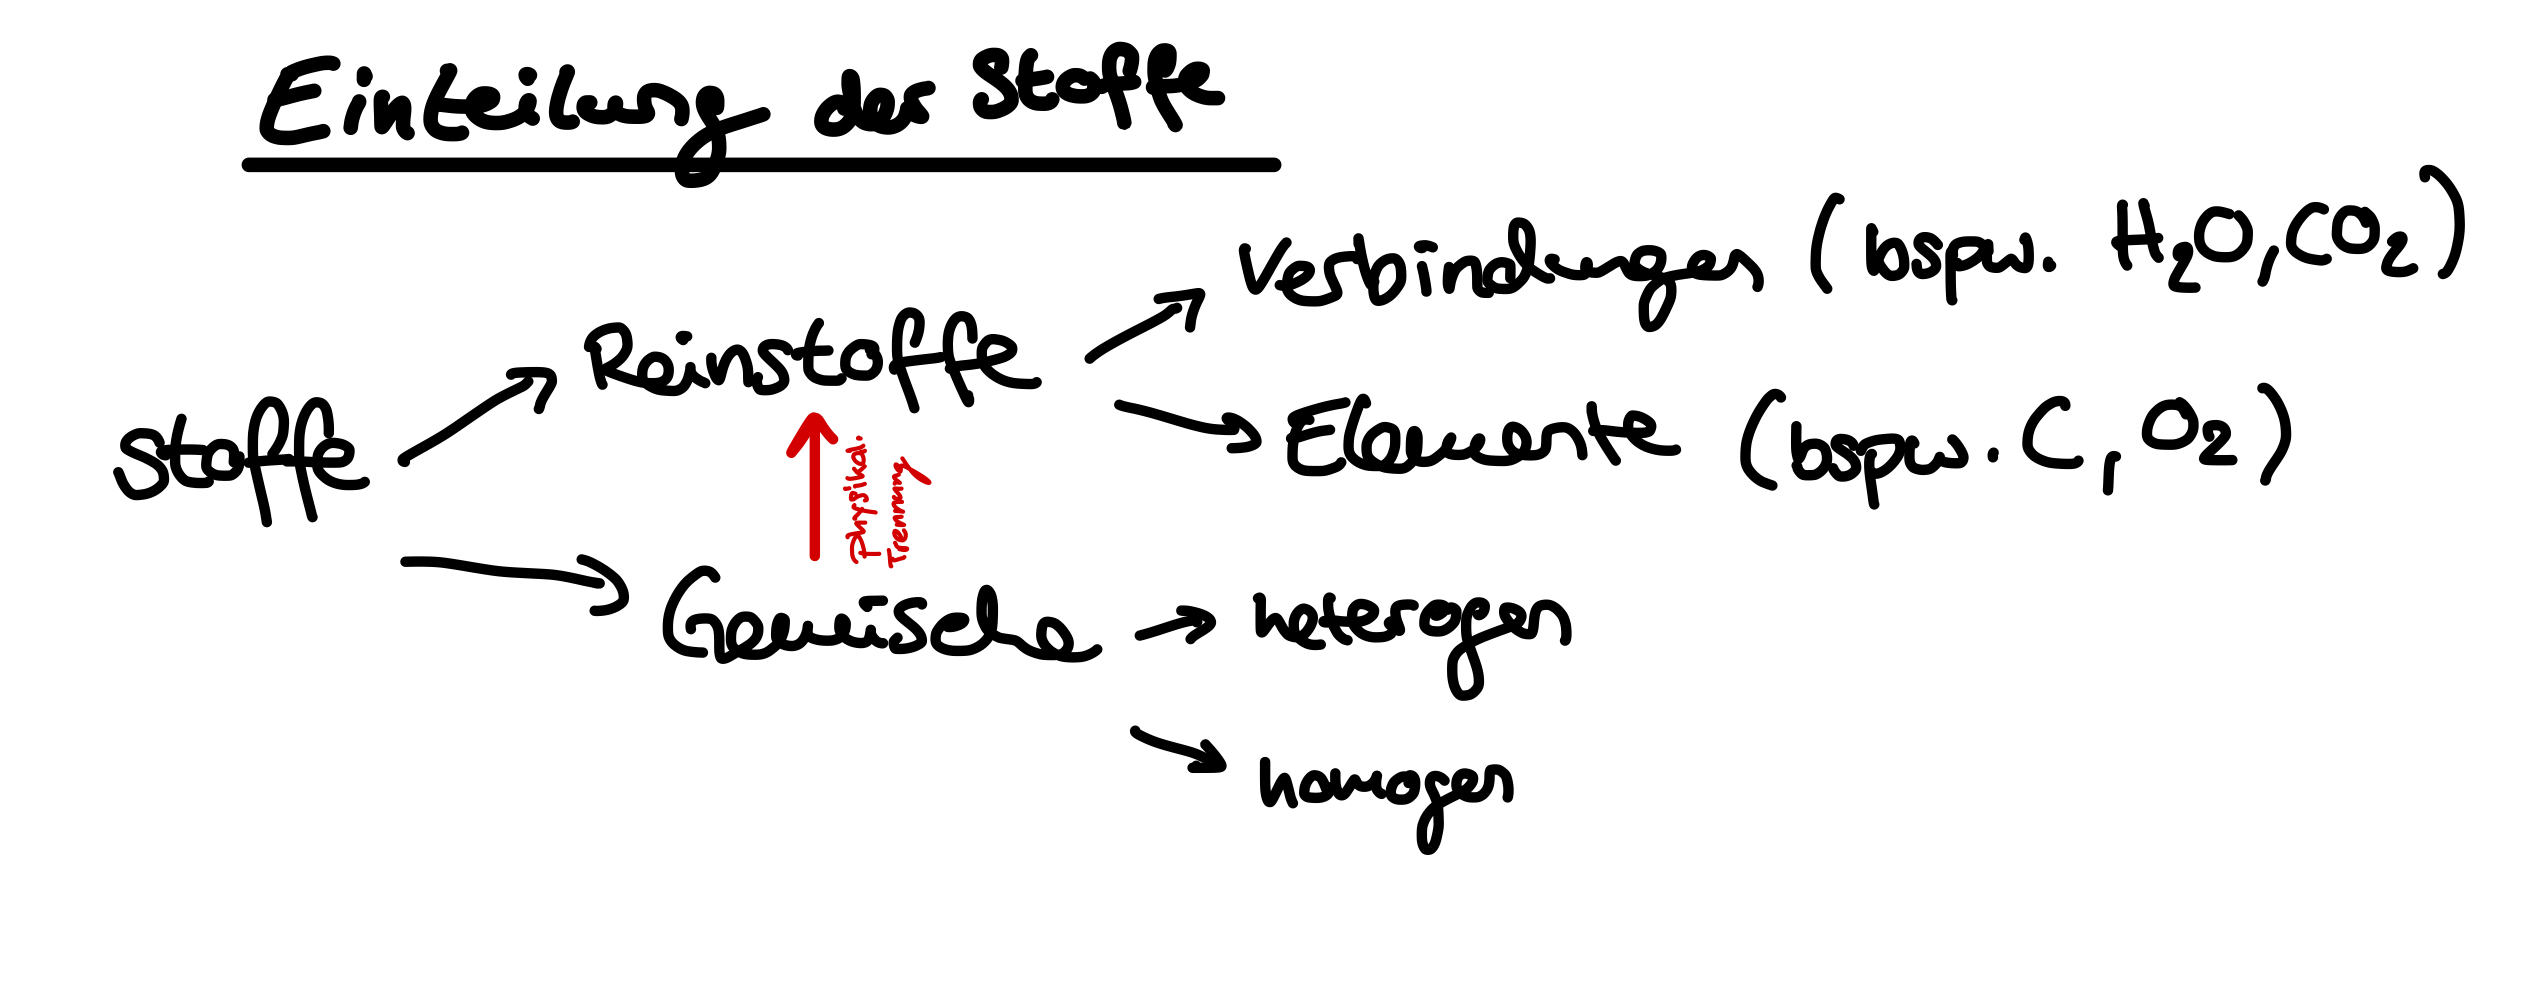
\includegraphics[width=9cm, height=3cm]{images/Stoffe.png}

\subsection{Aggregatzustand}		

{\tiny
\begin{tabular} {ll | ll} 
	Aggregatzustand  	&     					& Dispersitätsgrad    &  \\ 
	Dispersionsmittel  	& Dispergierter Stoff	& Heterogen   		& Homogen        \\
	gasförmig (g) 		& gasförmig (g)        	& -          		& Gasgemisch        \\
	gasförmig (g)		& flüssig (l)			& Nebel				& -		\\
	gasförmig (g)		& fest (s)				& Rauch				& -		\\
	flüssig (l)			& gasförmig (g) 		& wenig haltbarer Schaum	& Gaslösung		\\
	flüssig (l)			& flüssig (l) 			& wenig haltbare Emulsion				& Glüssigkeitslösung		\\
	flüssig (l)			& fest (s) 				& Suspension				& feststofflösung	\\
	fest (s)			& gasförmig (g) 		& fester Schaum ( zB. Schaumstoff)					&		\\
	fest (s)			& flüssig (l) 			& brei				&		\\
	fest (s)			& fest (s) 				& Feststoffgemische				& legierung zweier Metalle	\\
	
\end{tabular}
}

\subsection{Eselsbrücke}

\begin{tabular}{ll} 
    HONClBrIF – "der Brief vom Onkel"   &  Die Buchstaben stellen dabei \\
     & die Elemente des Periodensystems dar,\\
     & die in der Natur nur 2-atomig vorkommen. \\
    Ausnahme: & $P_4$ (Phosphor) und $S_8$ (Schwefel)  \\
\end{tabular}
\renewcommand{\arraystretch}{1}      
         

\subsection{Kugelwolkenmodell}	

\subsection{Isotope}

  
           
	\section{Stoffklassen}

\small{\begin{tabularx}{\columnwidth}{|l|l|l|X|}
	\hline
	\textbf{Stoffklasse} & \textbf{Bindungstyp} & \textbf{Beispiel} & \textbf{Eigenschaften} \\
	\hline
	Salze & Ionenbindung & NaCl, CaCl\textsubscript{2} & Spröde, \newline hohe Schmelzpunkte, lösen sich oft gut in Wasser \\
	\hline
	Metalle & Metallbindung & Cu, Fe, Al & Leitfähig, glänzend \\
	\hline
	Molekulare Stoffe & Kovalente Bindung & H\textsubscript{2}O, CO\textsubscript{2}, CH\textsubscript{4} & niedrige Schmelz- und Siedepunkte, oft gasförmig oder flüchtig \\
	\hline
\end{tabularx}}

\subsection{Bindungen}

\subsubsection{Elektronenpaar-Bindung}

Dieser Bindungstyp existiert ausschließlich bei \textbf{Nichtmetall}-Atomenverbänden. \newline Diese Atomverbände sind meist \textbf{Moleküle} (mit begrenzter Atom-Anzahl).

\textbf{Beispiele:} H\textsubscript{2}O, C\textsubscript{2}H\textsubscript{6} (Ethan), C\textsubscript{2}H\textsubscript{5}OH (Ethanol), NH\textsubscript{3} (Ammoniak)

\subsubsection{Metall-Bindung}

Dieser Bindungstyp tritt auf, wenn ausschließlich \textbf{Metall}-Atome den Atomverband bilden. Dieser besteht aus einem \textbf{Metallgitter} aus ``unendlich'' vielen Atomen.

\textbf{Beispiele:} Pb (Blei), Cu (Kupfer), Ag (Silber), Na (Natrium), Mg (Magnesium), Pd (Palladium)

\subsubsection{Ionen-Bindung}

Dieser Bindungstyp entsteht immer, wenn \textbf{Nichtmetall}-Atome mit \textbf{Metall}-Atomen reagiert haben. Er hält die bei der Reaktion gebildeten Ionen in einem Gitter aus ``unendlich'' vielen Ionen zusammen (= \textbf{Ionengitter}).

\textbf{Beispiele:} Na\textsuperscript{+}Cl\textsuperscript{--} (Natriumchlorid), Mg\textsuperscript{2+}Cl\textsubscript{2}\textsuperscript{--} (Magnesiumchlorid), K\textsuperscript{+}I\textsuperscript{--} (Kaliumiodid)


\subsection{Bindungswinkel}
\begin{center}
	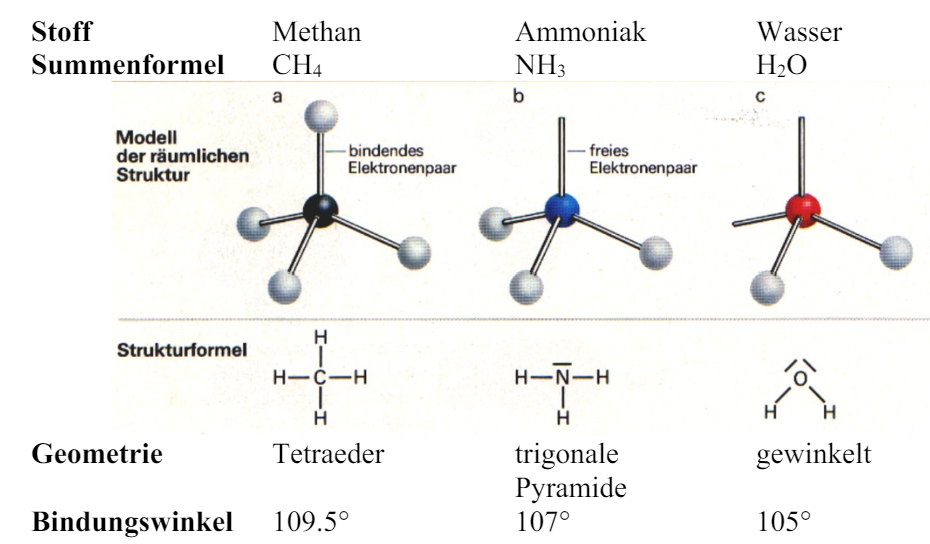
\includegraphics[height=4cm]{images/Winkel.png}
\end{center}

\subsection{Metalle und Halbmetalle}
 $\rightarrow$ Metalle besitzen durch delokalisierte Elektronenwolken (VE) dh. freie Ladungsträger, dies führt zu gute Wärme- und el. Leitfähigkeit, Verformbarkeit
\subsubsection {Leitfähigkeit bei Metallen}
	\begin{itemize}
		\item nimmt mit steigender Temperatur ab
		\item die Bewegung der Atomrümpfe erhöht sich
		\item weniger Platz für die Elektronenbewegung
	\end{itemize}
	
\begin{minipage}{0.48\columnwidth}
	\textbf{Beispiel Lithium:}
	\begin{itemize}
		\item Valenzband Vb nicht ganz gefüllt
		$\rightarrow$ Elektronen können sich im Band bewegen
	\end{itemize}
\end{minipage}
 \hfill
\begin{minipage}{0.48\columnwidth}
	\textbf{Beispiel Beryllium:}
	\begin{itemize}
		\item Valenzband komplett gefüllt, aber mit leerem Leitungsband überlappend
		$\rightarrow$ Elektronen können sich im Band bewegen
	\end{itemize} 
\end{minipage}
\begin{center}
	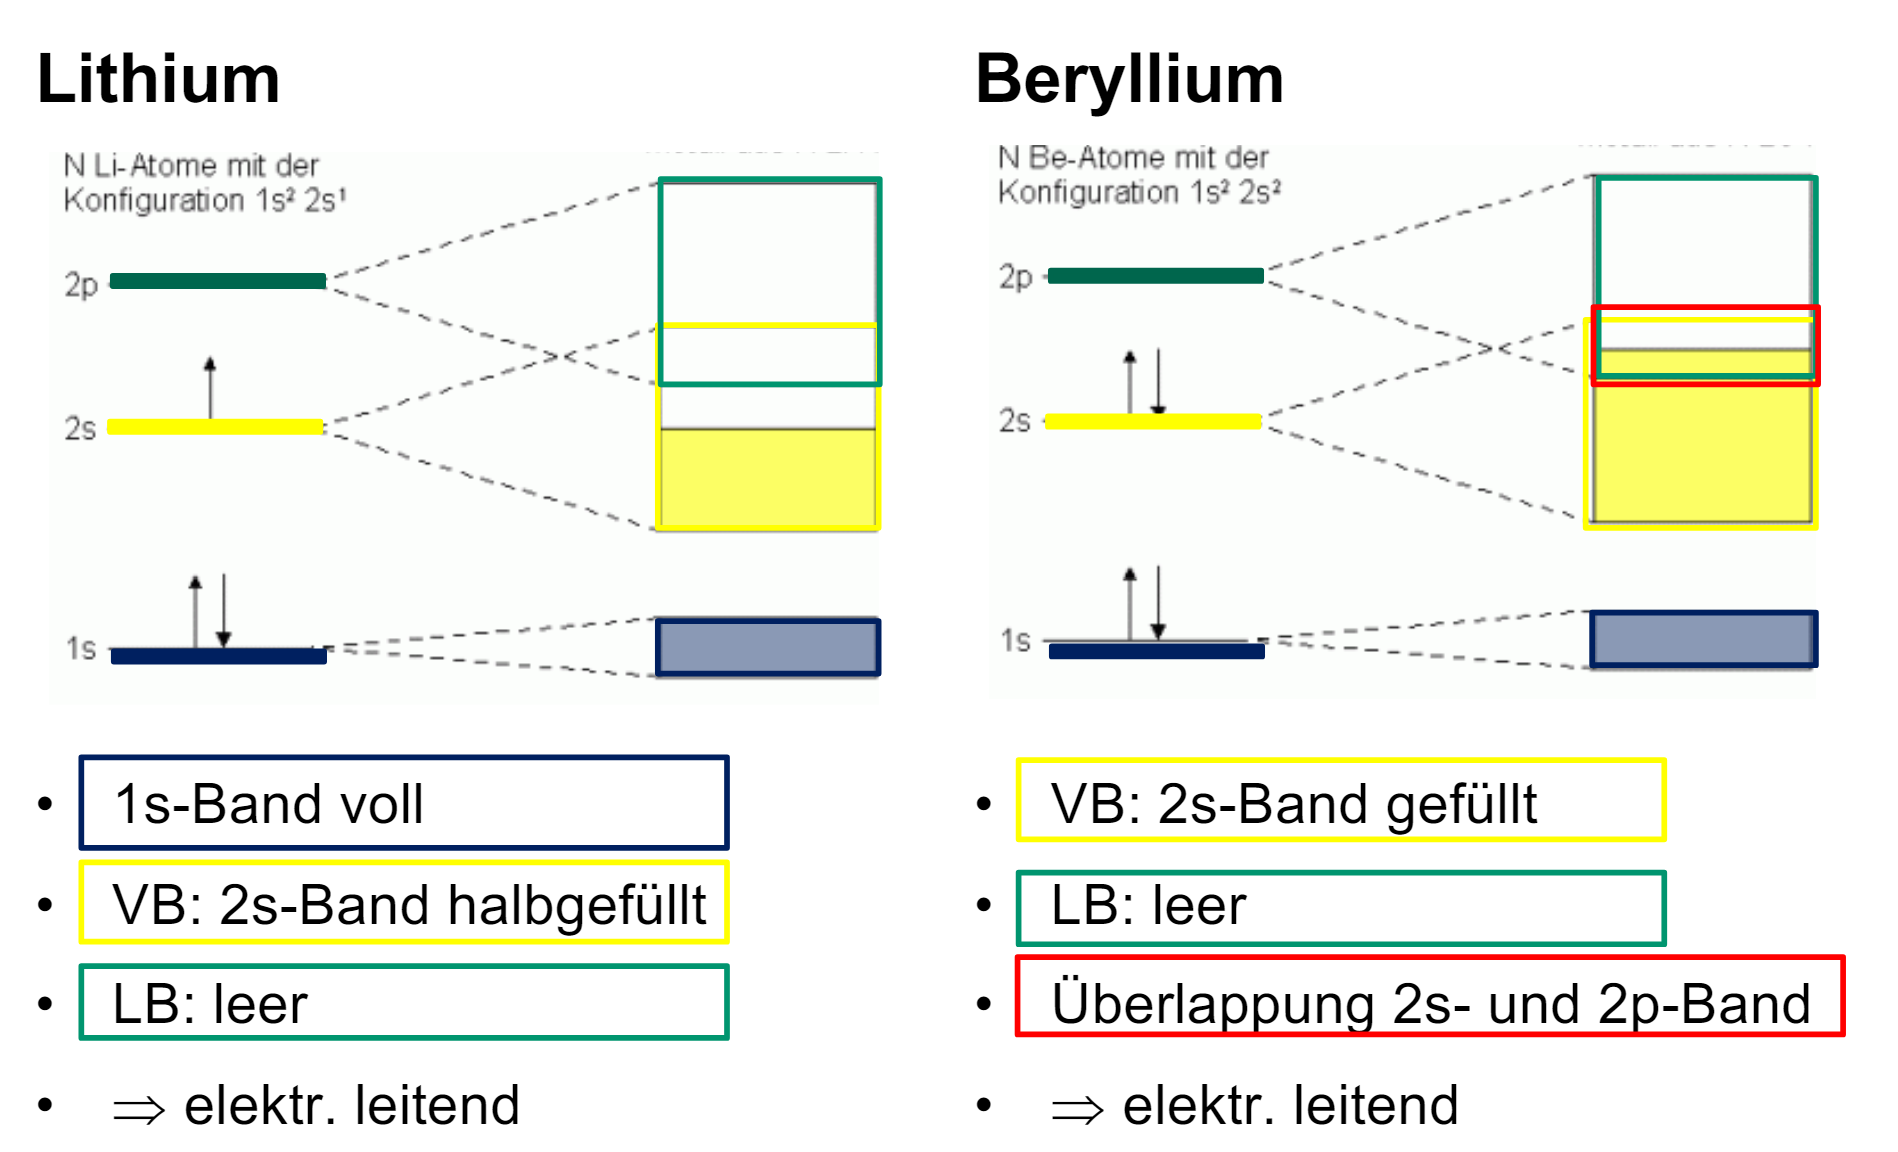
\includegraphics[height=3cm]{images/Baender.png}
\end{center}

 $\rightarrow$ Halbmetalle haben weder Elektronenwolken noch überlappende Energieniveaus, Nähe vom Valenz- und Leitungsband ermöglichen aber ein Überspringen
\subsubsection{Leitfähigkeit bei Halbmetallen}
	\begin{itemize}
		\item nimmt mit steigender Temperatur stark zu
		\item die Elektronen springen viel zahlreicher auf das Leitungband über
		\item Platz für Elektronenbewegung im Leitungsband
	\end{itemize}
	
\subsection{Dotierung von Halbmetallen}
Dotierung $\rightarrow$ Einbringen von Fremdatomen ins Atomgitter eines Halbleiters
\begin{itemize}
	\item \textbf{n-Halbleiter}
	\item[] z.B. einzelne As-Atome im Si-Gitter(1:10'000'000)
	\item[] Ein \tikz[baseline=(text.base)]\node[fill=orange, fill opacity=0.3, text opacity=1, rounded corners, inner sep=2pt, minimum height=5pt] (text) {\textit{überschüssiges}}; 
	Elektron pro As-Atom $\Rightarrow$ Leitfähigkeit: Elektron von As-Atom kann ins Leitungsband von Si überspringen und sich frei bewegen
	\item \textbf{p-Halbleiter}
	\item[] z.B. einzelne B-Atome im Si-Gitter(1:1'000'000)
	\item[] Ein \tikz[baseline=(text.base)]\node[fill=orange, fill opacity=0.3, text opacity=1, rounded corners, inner sep=2pt, minimum height=5pt] (text) {\textit{fehlendes}}; Elektron pro B-Atom $\Rightarrow$ Leitfähigkeit: Elektronen aus dem vollen Valenzband von Si können in diese ``Lücke'' springen und sich frei bewegen
\end{itemize}

	\section{Flüssigkristalle}

\subsection{Inhalt}
\begin{itemize}
\item Definition
\item  Atomarer Aufbau
\item flüssigkristalline Phasen
\item TN-Zellen
\end{itemize}

\subsection{Definition}

\subsection{Molekülstruktur}

\subsection{TN-Zelle (Twisted Nematic)}
\begin{minipage}{0.48\linewidth}
	\begin{center}
		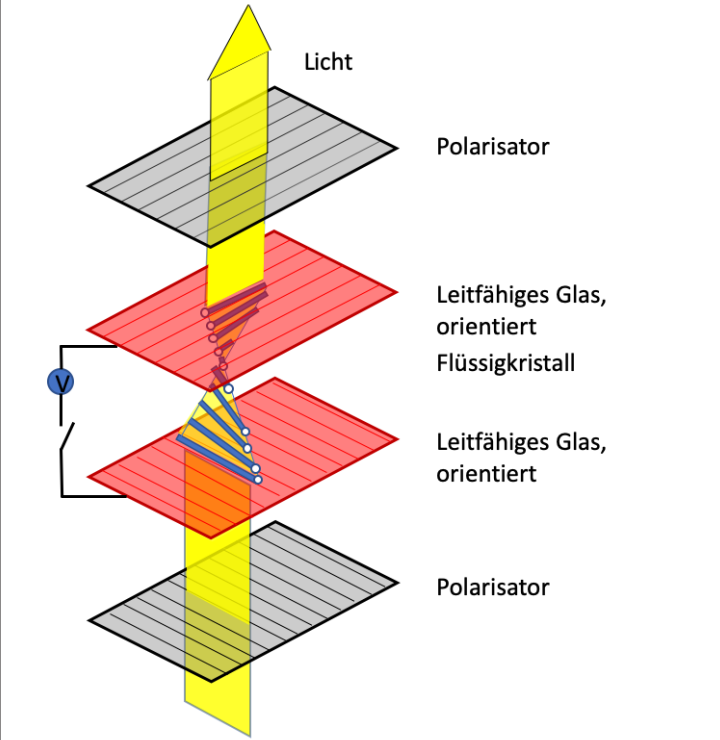
\includegraphics[width=0.8\linewidth]{images/TN-Zelle1.png}
		
		ohne angelegte Spannung   
	\end{center}
\end{minipage}
\hfill
\begin{minipage}{0.48\linewidth}
	\begin{center}
		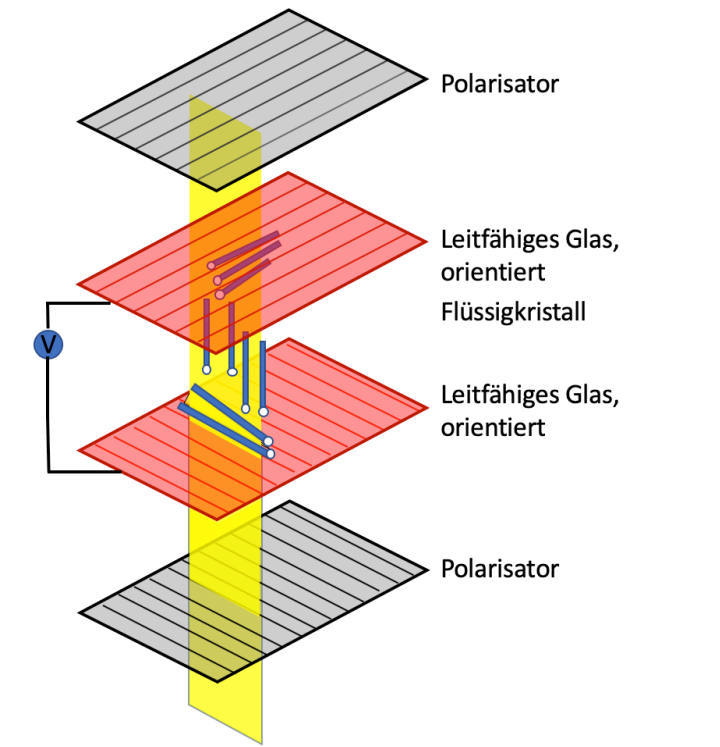
\includegraphics[width=0.8\linewidth]{images/TN-Zelle2.png} 
		
		mit angelegter Spannung 
	\end{center}
\end{minipage}

	\section{Ablauf chemischer Reaktionen}

\subsection{Thermochemie}
\subsubsection{Enthalpie}
Beschreibt den Wärmeinhalt eines Systems, Prinzip Energieminimum:
$$\boxed{\Delta H_R = H_{Produkte} - H_{Edukte}} $$
\begin{tabular}{l l}
	$\Delta H_R < 0 \text{ \textbf{exotherm}, Energie wird frei}$ & $\Delta H_R > 0 \text{ \textbf{endotherm}, Energie wird aufgenommen}$ \\
	$\text{[H]} =\frac{J}{mol}$ & \\
\end{tabular}
\subsubsection{Entropie}
Beschreibt verschiedene Anordnungsmöglichkeiten von Teilchen in einem System,\break Prinzip Energiemaximum:
$$\boxed{\Delta S_R = S_{Produkte} - S_{Edukte}} $$
\begin{tabular}{l l}
	$\Delta S_R < 0 \text{  \textbf{Unordnung nimmt ab} z.B. wenn Gase zu Flüssigkeit reagieren}$ &  \\
	$\Delta S_R > 0 \text{  \textbf{Unordnung nimmt zu} z.B. wenn ein Feststoff zu Gas wird}$     &  \\
	$\text{[S]}=\frac{J}{mol \cdot K}$                                                            & \\
\end{tabular}

\subsubsection{Freie Enthalpie}
Gibbs-Helmholtz-Gleichung definiert, ob eine Reaktion bei konstanter Temperatur und konstantem Druck freiwillig (spontan) verlauft:
$$\boxed{\Delta G = \Delta H - T \cdot \Delta S} $$
\begin{tabular}{l l}
	$\Delta G < 0 \text{  \textbf{freiwillig} Exergon}$    &  \\
	$\Delta G > 0 \text{  \textbf{unfreiwillig} Endergon}$ &  \\
	$\text{[G]}=\frac{J}{mol}$                             & \\
\end{tabular}

\subsection{Reaktionsgeschwindigkeit}

$$ \boxed{\text{RGT-Faustregel:}\pm T=\pm 10^{\circ}C \rightarrow  \text{um Faktor 2 erhöhen oder senken (in d, h, min)}}$$

Chemische Reaktionen benötigen eine Aktivierungsenergie. \newline 
Diese sagt aus, wie schnell die Reaktion passiert.
Exotherme Reaktionen verlaufen nach anfänglicher Aktivierung oft freiwillig.

\subsubsection{Katalysatoren}
\label{Reaktionsgeschw}
\begin{minipage}{0.2\linewidth}
	% \vspace*{0pt}
	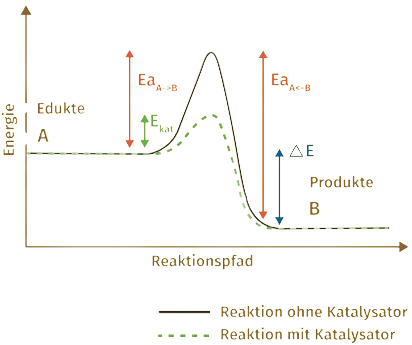
\includegraphics[width=\linewidth]{images/Katalysator_1.png}
\end{minipage}
\hfill
\begin{minipage}{0.65\linewidth}
	\begin{itemize}
		\item Katalysator = Stoff nimmt an Reaktion teil, wird nicht verbraucht 
		\item Beschleunigt Reaktion: $E_{AKat} \ll E_{ANorm}$
		\item $\Delta$ G sowie $\Delta H_R$ bleiben gleich
		\item Selektiv (wirkt nicht mit allen Stoffen)
	\end{itemize}
\end{minipage}


	\section{Säure, Basen und pH-Wert} {SW 7}

\subsection{Inhalt}
\begin{itemize}
\item Definition
\item Protolysen
\item Säure-Base-Reihe GGW (lese beschreibung!)
\item pH-Wert
\item  neutralisation
\end{itemize}

\subsection{Bedeutung}

\subsection{Säure-Base GGW}
\begin{minipage}{0.65\columnwidth}
	Bergab = GGW rechts: \ce{ HCl + H2O <=>> Cl- + H3O+ }
	
	Bergauf = GGW links: \ce{ HS- + H2O <<=> S^{2-} + H3O+ }
\end{minipage}
    \section{Redox-Reaktionen} {SW 10-13}

\subsection{Inhalt}
\begin{itemize}
\item Definitionen
\item  Oxidationszahlen
\item Redoxreihe
\end{itemize}

    \section{Korrosion}
\subsubsection{Definition}
Reaktion eines (metallischen) Werkstoffs mit seiner Umgebung, die zu messbaren Veränderungen des Werkstoffs (Ladung / Oxidation) und zu \textbf{Korrosionsschäden} führen kann. \newline
Metall reagiert als RM: \ce{Me <--> $Me^{z+}$ + z e-}
Möglich wenn $\Delta$G $<$ 0 $\&$ v.a. \ce{O2, H2O/H3O+} (OM) vorhanden. \newline
Spalt = kleine Anode, Passivoxidschicht = grosse Kathode \newline
Wenn $E_a$ gross $\to$ Reaktionsgeschwindigkeit klein

\subsection{Korrosionstypen}
\small{
\subsubsection{Elektrochemische Korrosion}
	Häufigste Korrosionsart, Ox. und Red. \textbf{räumlich getrennt}, wässriger Elektrolyt. \newline
	$\Rightarrow$ Bildung galvanische Zelle


\subsubsection{H2 und O2 Typ Korrosion}
\begin{tabular}{ll}
	H2 & OM ist $H^+$, pH abhängig \\
	\textbf{Beispiel} & \\
	Sauer: & \ce{2H3O+ + 2 e- <--> H2 + 2H20} \\
	neut.-Bas.: & \ce{2H2O + 2 e- <--> H2 + 2 OH-} \\
	& \\
	O2 & OM ist O2, pH-abhägig, je saurer die Lösung, desto aggressiver korrodiert. \\
	\textbf{Beispiel} & \ce{O2 + 2H2O + 4e- -> 4OH-} \\
	& \ce{2Fe + 3/2 O2 + H2O -> 2FeOOH}
\end{tabular}
\smallskip

\textbf{Potentialverhältnisse: Bedingung zur Korrosion von H2 und O2} \newline
$\rightarrow E(M/M^+)$ und $E(OM)$ abhängig \newline
$\rightarrow \Delta G < 0$  \newline
$\boxed{E(OM) = E_{H2} = -0.059V \cdot pH ~~ \text{und} ~~ E_{O2}= 1.23 - 0.059V \cdot pH}$ 
\smallskip \newline
$\boxed{
	E_{\ce{Me / Me^{n+}}} = E^\circ_{\ce{Me / Me^{n+}}} + \frac{0.06\,\mathrm{V}}{z} \cdot \lg [\ce{Me^{n+}}]}$

\subsubsection{Eisen (Rost)}
Korrosion von Eisen-Werkstoffen mit O2 und H2O  OM ist O2, feuchtigkeit abhängig, Ionengehalt verstärken

\subsubsection{Kontaktkorrosion, Bimetallkorrosion}
Korrosion eines unedleren Metalls, das mit einem edleren Metalle elektrisch und via wässrigem Elektrolyten verbunden ist.
Reduktion von \ce{O2} an gesamter Oberfläche, Oxidation nur an unedlerem Metall $\rightarrow$ verstärkte Korrosion, Edleres Metall $\rightarrow$ keine Korrosion (kathodisch geschützt) \newline
 Flächenregel: $\frac{v_k(Zn)}{v_k(Zn + Fe)} = \frac{A(Zn)}{A(Zn + Fe)} = \frac{\text{Anodenfläche}}{\text{Kathodenfläche}}$ \newline 
$\rightarrow$ Je grösser die Fläche des edleren Metalls, umso schneller korrodiert das unedlere

\subsubsection{gleichmässige Flächenkorrosion}
Auflösung ist gleichmässig über gesamte Metalloberfläche verteilt. 

\subsubsection{Lochfrass-Korrosion}
stark lokalisierte Korrosion, Bildung enger, tiefer Löcher – Verhältnis(Durchmesser/Tiefe) < 1, Materialabtrag gering \newline 
$\rightarrow$ gefährlich, da schwer erkennbar – kann innert kurzer Zeit zur Durchlöcherung führen

\subsubsection{Belüftungselemente}
Korrosion infolge räumlich variierendem O2-Gehalt im Elektrolyten, können Lochfrasskorrosion bewirken, lokale Depassivierung, inkl. Spaltkorrosion

}

\subsection{Passivatoren und Depassivatoren}
Passivator bildet an Oberfläche eine schützende Oxidschicht ($E_A$ wird vergrössert) \newline
Depassivator zerstört schützende Oxidschicht durch $\ce{Cl^-}$ ($E_A$ wird verkleinert)

    \section{Anhang}

\subsection{praktische Anwendungen der Redox Reaktionen}
\subsubsection{galvanische Zelle}
\subsubsection{Batterien und Akkus}
\subsubsection{Brennstoffzellen}
\subsubsection{elektrolytische Verfahren}
    \end{layout}
\end{document}
